
%+++++++++++++++++++++++++++++++++++++++++++
\section{The Maximum Entropy Principle}
%-------------------------------------------

Suppose that $p_1$ and $p_2$ are probabilities for independent events, the 
information $I$ received from seeing both events is the information of seeing 
each event added together.
$$
I(p_1p_2) = I(p_1) + I(p_2).
$$
\noindent{}See if you can deduce why these criteria imply that the information 
of an event with probability $p$ can be suitably defined as 
$I(p) \equiv \log \frac{1}{p}$.
\noindent{}The Shannon entropy $\mathcal{H}$ is compactly defined as the 
expected information content of a random variable $X$:
$$
\mathcal{H}(X) \equiv \mathbb{E}_{x\sim X}\left[I(p(x))\right].
$$
\noindent{}For simplicity, here we supress details about differential entropy, 
which defines entropy for continuous random variables. For our purposes, the 
equation above applies to any random variable.


%+++++++++++++++++++++++++++++++++++++++++++
\subsection{Information, Shannon Entropy, Cross-Entropy, KL divergence}

“{\bf 信息}”,对概率分布 $p(x)$ 取对数加符号得正值:
$$
I(p) = -\log p(x)
$$
概率越高,包含的信息小,因为事件越来越确定。相反,概率越低,包含的信息越多,因为事件具有很大的不确定性。

“{\bf 熵/Shannon entropy}”,用来描述系统中所含信息的不确定程度(系统的混乱程度):
\begin{align}\label{entropy_of_info}
H(p) 
&\equiv \mathbb{E}_{x\sim P}\left[I(p)\right] \notag \\
&= - \sum p(x) I(p) \notag \\
&= - \sum p(x) \log p(x)
\end{align}
熵是信息的平均,直观上,Shannon熵是信息在{\bf 同一分布}下的平均。
在公式\eqref{entropy_of_info}中,如果$\log$以2为底数,熵的单位就是比特(bit);
以10为底数的话单位则是哈特(hat);而如果是自然对数,单位则是奈特(nat)。

“{\bf 信息量}”,用来衡量一个事件的不确定程度:一个事件发生的概率越大,不确定性越小,
则它所携带的信息量就越小。假设$X$是一个离散型随机变量,其取值集合为$X$,概率分布函数为
$p(x)=P(X=x)$,$x\in X$。我们定义事件$X=x_0$的信息量为:
$I(x_0) = -\log(p(x_0))$。当$p(x_0)=1$时,熵将等于$0$,
也就是说该事件的发生不会导致任何信息量的增加。

可以看到,{\bf 熵是一个系统中信息量的总和}。

【{\bf 例}】

假如某项打靶运动的结果是一个0-1分布,其分布$X$的取值有{0:打中,1:脱靶}。
假设小明和小王在这项打靶运动中打中的先验概率为10%,99.9%。
根据上面的信息量的介绍,我们可以分别得到小明和小王打靶打中的信息量。
如果我们想进一步度量小明打靶结果的不确定度,就可以用熵的概念。
可以采用期望来进行度量,即对所有可能事件所带来的信息量求期望,其结果就能衡量小明打靶的不确定度:
\begin{align*}
H_A(x) &= - \left[ p(x_A)\log p(x_A) + (1-p(x_A))\log(1-p(x_A)) \right] \\
&= 0.4690
\end{align}
与之对应的,小王的熵(打靶的不确定度)为:
\begin{align*}
H_B(x) &= - \left[ p(x_B)\log p(x_B) + (1-p(x_B))\log(1-p(x_B)) \right] \\
&= 0.0114
\end{align}

虽然小明打靶结果的不确定度较低,毕竟十次有9次都脱靶(即脱靶的确定性高、不确定性低);
但是小王打靶结果的不确定度更低,1000次射击只有1次脱靶,结果相当的确定。


%+++++++++++++++++++++++++++++++++++++++++++
\subsection{最大熵原理}
最大熵原理中蕴含着最朴素最简洁的思想:包含已知信息,不做任何未知假设,把未知事件当成概率事件处理。

\begin{emp_box}
{\bf 最大熵原理:}

1. 满足已知信息(约束条件)

2. 不做任何未知假设(剩下的等概率)
\end{emp_box}

{\bf 熵表示不确定程度,熵最大即系统的不确定程度最大,亦即系统中没有任何主观假设。}


%+++++++++++++++++++++++++++++++++++++++++++
\subsection{Cross Entropy}

{\bf 交叉熵}
主要刻画的是实际输出(概率)与期望输出(概率)的距离,也就是交叉熵的值越小,
两个概率分布就越接近。假设概率分布$p$为期望输出,概率分布$q$为实际输出, 
$H(p,q)$为交叉熵,则
\begin{align}\label{Cross_Entropy}
H(p,q) 
&\equiv \mathbb{E}_{x\sim P}\left[I(q)\right] \notag \\
&= - \sum p(x) I(q) \notag \\
&= -\sum_x\left[ p(x)\log q(x) + (1-p(x))\log (1-q(x)) \right]
\end{align}
熵是信息{\bf 在同一分布下}的平均,而交叉熵是信息{\bf 在不同分布下}的平均。

\begin{example}
假设$N=3$,期望输出为$p={1,0,0}$,实际输出$q_1=(0.5,0.2,0.3)$, 
$q_1=(0.8,0.1,0.1)$,那么:
\begin{align*}
H(p,q_1) &= -(1\log0.5 + 0\log0.2 + 0\log0.3 + 0\log0.5 + 1\log0.8 + 1\log0.7) 
&= 0.55 \\
H(p,q_2) &= -(1\log0.8 + 0\log0.1 + 0\log0.1 + 0\log0.2 + 1\log0.9 + 1\log0.9) 
&= 0.19
\end{align}
通过上面可以看出,$q_2$与$p$更为接近,它的交叉熵也更小。
\end{example}


\subsubsection{机器学习中的交叉熵}

我们将KL散度定义公式(\ref{Kullback-Leibler_Divergence})进行如下变形:
\begin{align*}
D(P||Q) &= \sum_{x\in X} P(x)\log\frac{P(x)}{Q(x)} \\
&= \sum_{x\in X} P(x)\log P(x) - \sum_{x\in X} P(x)\log Q(x) \\
&= - H(P(x)) + \left[ \sum_{x\in X} P(x)\log Q(x) \right]
\end{align}
最后结果的前面一项就是$P$的熵,而等式后一项则是机器学习中常用的交叉熵:
\begin{equation}\label{Cross_Entropy_Loss}
L(P,Q) = -\sum_{x\in X} P(x)\log Q(x)
\end{equation}
在机器学习中,我们需要评估label和predicts之间的差距,使用KL散度$D(P||Q)$刚刚好。
由于KL散度中的前一部分$−H(P(x))$不变,故在优化过程中,
只需要关注后一项交叉熵$L(P,Q)$就可以了。
所以一般在机器学习中直接用用交叉熵做loss来评估模型。


\subsubsection{Pytorch中的CrossEntropyLoss()函数}

Pytorch中计算的交叉熵并不是采用(\ref{Cross_Entropy}),
而是使用(\ref{Cross_Entropy_Loss})中的公式:
它是机器学习中常使用的另一种方式的交叉熵。此小节之前的那个小节最后已经为此做了说明。

% https://zhuanlan.zhihu.com/p/98785902

由于KL散度中的前一部分$−H(P(x))$不变({\bf 目标分布的熵为常数}),故在优化过程中,
只需要关注交叉熵就可以了。但是如果目标分布是有变化的(如同为猫的样本,不同的样本,
其值也会有差异),{\bf 那么就不能使用交叉熵}。例如蒸馏模型的损失函数就是KL散度,
因为蒸馏模型的目标分布也是一个模型,该模型针对同类别的不同样本,
会给出不同的预测值(如两张猫的图片a和b,目标模型对a预测为猫的值是0.6,对b预测为猫的值是0.8)。

% https://blog.csdn.net/qq_43742590/article/details/115483032

{\bf 不直接用距离相关的均方差:}

假设神经网络的最后一层激活函数为sigmoid,它的两头异常的平,也就是说在那些地方的导数接近于0。
而反向传播是需要求导的,用了均方差损失函数之后求导结果包含$y(y-1)$ ,
$y$接近于$0$或者$1$的时候都趋于$0$,会导致梯度消失,网络训练不下去(梯度弥散)。
但如果用相对熵衍生出来的交叉熵作为损失函数则没有这个问题。
因此虽然相对熵的距离特性不是特别好,但总归好过直接梯度消失玩不下去,
因此很多用sigmoid作为激活函数的神经网络还是选择了用相对熵衍生出来的交叉熵作为损失函数。


{\bf 多使用交叉熵:}

针对以上不足,有两个方向来避免,一是从激活函数下手,一是从损失函数下手。
这里我们不换激活函数,还是用sigmoid函数,引入了交叉熵损失函数:
$$
L = \sum_i\left[ z_i\ln y_i + (1-z_i)\ln(1-y_i) \right]
$$
这时再看权重更新公式:
$$
\frac{\partial L}{\partial w_{ji}} 
= \frac{\partial L}{\partial \text{node}_j}\frac{\partial \text{node}_j}{\partial w_{ji}}
= \frac{\partial L}{\partial \text{node}_j}\frac{\partial \Sigma_i w_{ji}x_{ji}}{\partial w_{ji}}
= \frac{\partial L}{\partial \text{node}_j}x_{ji}
$$
此时对于输出层,权重更新公式为:
$$
\frac{\partial L}{\partial w_{ji}} 
= \frac{\partial L}{\partial y_j}\frac{\partial y_j}{\partial \text{node}_j}x_{ji}
= x_{ji}(z_j-y_j)
$$
可以看到梯度下降已经不与sigmoid的导数相关了,而是由误差来影响。
当误差较大时则下降较快,让梯度下降法更有效率,避免了训练慢的问题。
与sigmoid的导数无关,从而避免了梯度弥散。


%+++++++++++++++++++++++++++++++++++++++++++
\subsection{Lagrange乘数法的几何意义说明}

\begin{emp_box}
{\bf Lagrange乘数法:}
\begin{align*}
&\max f(x,y) \\
&\text{约束条件:} g(x,y) = 0
\end{align}
\end{emp_box}

对于一般的求极值问题我们都知道,求导等于0就可以了。但是如果我们不但要求极值,
还要求一个满足一定约束条件的极值,那么此时就可以构造Lagrange函数,
其实就是把约束项添加到原函数上,然后对构造的新函数求导。
看下面的图就很容易理解了。

\begin{figure}[H]
\centering
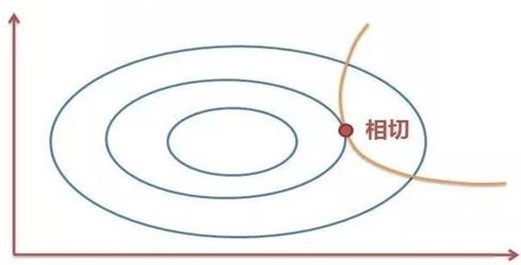
\includegraphics[scale=0.7]{pix/lagrange.jpg}
\caption{Lagrange乘数法}
%\label{fig:label}
\end{figure}

对于一个要求极值的函数$f(x,y)$,图上的蓝圈就是这个函数的等高图,就是说
$f(x,y)=C_1,C_2,\cdots,C_n$分别代表不同的数值(每个值代表一圈,等高图)。
现在要找到一组(x,y),使它的$C_i$值越大越好,但是这点必须满足约束条件
$g(x,y)$(在黄线上)。

也就是说$f(x,y)$和$g(x,y)$相切,或者说它们的梯度$\nabla f$和$\nabla g$平行,
因此它们的梯度(偏导)成倍数关系(假设为$\lambda$倍)。
故而把约束条件加到原函数后再对它求导,其实就等价于满足下面的式子:
\begin{align*}
\frac{\partial f}{\partial x} &= \lambda \frac{\partial g}{\partial x} \\
\frac{\partial f}{\partial y} &= \lambda \frac{\partial g}{\partial y}
\end{align}


%+++++++++++++++++++++++++++++++++++++++++++
%\subsection{Relative Entropy (Kullback-Leibler Divergence / Information gain)}
\section{KL Divergence for Machine Learning \\
{\small Relative entropy / Information gain}}
%-------------------------------------------
% https://dibyaghosh.com/blog/probability/kldivergence.html
% \href{https://blog.csdn.net/wangshun_410/article/details/84956539}{KL距离(Kullback-Leibler Divergence)}
\begin{emp_box}
The objective of life is just to minimize a KL objective.
\end{emp_box}

Here in this section we talk about the {\bf Kullback-Leibler Divergence} from a holistic 
perspective of reinforcement learning and machine learning. Put simply, the KL divergence 
between two probability distributions measures how different the two distributions are.
KL 距离,是Kullback-Leibler差异(Kullback-Leibler Divergence)的简称,
也叫做相对熵(Relative Entropy)。它衡量的是相同事件空间里的两个概率分布的差异情况。
并不是一种距离度量方式,其物理意义是:在相同事件空间里,概率分布$p(x)$对应的每个事件,
若用概率分布$q(x)$编码时,平均每个基本事件(符号)编码长度增加了多少比特。
\begin{emp_box}\noindent
Both the problems of supervised learning and reinforcement learning are simply minimizing 
the KL divergence objective
\end{emp_box}


%+++++++++++++++++++++++++++++++++++++++++++
\subsection{What's the KL Divergence?}

The Kullback-Leibler divergence (hereafter written as KL divergence) is a measure of how 
a probability distribution differs from another probability distribution. Classically, 
in Bayesian theory, there is some true distribution $p(X)$; we'd like to estimate with 
an approximate distribution $q(X)$. In this context, the KL divergence measures the 
distance from the approximate distribution $q$ to the true distribution $p$.

Mathematically, consider two probability distributions $p$, $q$ on some space $\mathcal{X}$. 
The Kullback-Leibler divergence from $q$ to $p$ (written as $D_{KL}(p \| q)$ or simply 
$D(p \| q)$):
\begin{align}
D(p\|q) 
&\equiv \mathbb{E}_{x \sim p}\left[\log \frac{p(X)}{q(X)}\right] 
\label{Kullback-Leibler_Divergence_expec}\\
&= H(p,q) - H(p) \notag \\
&= \sum p(x)\log q(x) + \sum p(x) \log p(x) \notag \\
&= -\sum_{x\in X} p(x)\log\frac{q(x)}{p(x)} \notag \\
&= \sum_{x\in X} p(x)\log\frac{p(x)}{q(x)}\label{Kullback-Leibler_Divergence}
\end{align}
【{\bf 注记}】

There are some immediate notes that are worth pointing out about this definition.
若 $p$ 表示样本的真实分布,$q$ 表示模型所预测的分布,那么 KL 散度就可以计算两个分布的差异,
也就是 Loss 损失值。$q$ 的分布越接近 $p$($q$ 分布越拟合 $p$),那么散度值越小,即损失值越小。
~\\	%一行空白

有时会将KL散度称为KL距离,但它并不满足距离的性质(下面的4及5)。
由公式(\ref{Kullback-Leibler_Divergence})可以知道如下性质:
%
\begin{itemize}
%\setlength{\itemsep}{0pt}
%\setlength{\parsep}{0pt}
\setlength{\parskip}{0pt}
\item[1.]
当$p(x)=q(x)$时,$D(p||q)=0$,即其相对熵为零;

\item[2.]
当$p(x)$和$q(x)$相似度越高时,KL距离越小;

\item[3.]
$D(p \| q)$非负:
\begin{align*}
-D(p||q)
&= \sum p(x)\log\frac{q(x)}{p(x)} \\
&\leq \log \sum p(x) \frac{q(x)}{p(x)} \\
&= \log 1 \\
&= 0
\end{align}
上面使用了 Jensen's inequality.

\item[4.]
The KL Divergence is {\bf not symmetric}:
$$
D(p \| q) - D(q \| p) = \sum(p(x) + q(x))\log\frac{p(x)}{q(x)}
$$
and hence $D(p \| q) \neq D(q \| p)$.
The KL Divergence can take on values in $[0,\infty]$.
Particularly, if $p$ and $q$ are the exact same distribution 
($p \stackrel{a.e.}{=} q$), then $D_{KL}(p \| q) = 0$ and $D_{KL}(q \| p) = 0$.
In fact, with a little bit of math, a stronger statement can be proven: if 
$D_{KL}(p \| q) = 0$, then $p \stackrel{a.e.}{=} q$.

In order for the KL divergence to be finite, the support of $p$ needs to be contained in 
the support of $q$. If a point $x$ exists with $q(x) = 0$ but $p(x) > 0$, then 
$D_{KL}(p \| q) = \infty$.

\item[5.]
convexity - concave:
\begin{align*}
& D\left[ \lambda p_1(x) + (1-\lambda)p_2(x) || \lambda q_1(x) + (1-\lambda)q_2(x) \right] \\
= & \sum\left[\lambda p_1(x) + (1-\lambda)p_2(x)\right]\log
\frac{\lambda p_1(x) + (1-\lambda)p_2(x)}{\lambda q_1(x) + (1-\lambda)q_2(x)} \\
\leq & \sum\left[ \lambda p_1(x)\log\frac{\lambda p_1(x)}{\lambda q_1(x)} 
+ (1-\lambda)p_2(x)\log\frac{(1-\lambda)p_2(x)}{(1-\lambda)q_2(x)} \right] \\
= & \lambda D[p_1(x)||q_1(x)] + (1-\lambda)D[p_2(x)||q_2(x)]
\end{align}
上面的不等式用到了 \href{https://statproofbook.github.io/P/logsum-ineq}{log sum inequality}.

\item[6.]
不满足三角不等式。Since the KL Divergence is not symmetric, it is also {\bf not a distance metric}.

\item[7.]
{\bf Rewriting the Objective:} With some algebra, we can manipulate the definition of KL 
divergence in terms of other quantities. The most useful such manipulation is:
$$
D_{KL}(p \| q) = \mathbb{E}_{x \sim p}[-\log q(x)] - \mathcal{H}(p(x))
$$
Here, $\mathbb{E}_{x \sim p}[-\log q(x)]$ is the cross entropy between $p$ and $q$ (and 
denoted $H(p,q)$). The second term $\mathcal{H}(p(x))=\mathbb{E}_{x \sim p}[-\log p(x)]$ 
is the entropy of $p$.

\end{itemize}
%~\\ 
%~\\[0.2]	%可加入任意间距的空白行
~~~


%+++++++++++++++++++++++++++++++++++++++++++
\subsection{Forward and Reverse KL}

Let's place ourselves in the optimization setting. There is some true distribution 
$p(X)$ that we're trying to estimate with our approximate distribution $q_\theta(X)$. 
Here we are using $\theta$ as a parameter to explicitly emphasize that $q$ is the 
distribution that we get to control.

As we mentioned earlier, the KL divergence is not a symmetric measure (i.e. that 
$D_{KL}(p \| q) \neq D_{KL}(q \| p)$). As a result, when trying to approximate $p$, 
we have a choice between two potential objectives to optimize.
%
\begin{itemize}
%\setlength{\itemsep}{0pt}
%\setlength{\parsep}{0pt}
\setlength{\parskip}{0pt}
\item[1.]
Minimizing the {\bf forward KL}: $\arg\min_{\theta} D_{KL}(p\|q_\theta)$

\item[2.]
Minimizing the {\bf reverse KL}: $\arg\min_{\theta} D_{KL}(q_\theta\|p)$

\end{itemize}
As it turns out, the two different objectives actually cause different types of 
approximations. We'll spend the next subsection discussing the qualitative behaviours of 
each approach. We'll investigate in the following setting: $p(X)$ is the bimodal 
distribution below. We'll try to approximate this with a normal distribution 
$q(X) = \mathcal{N}(\mu, \sigma^2)$.

\begin{figure}[H]
\centering
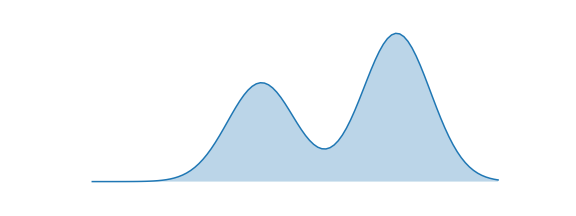
\includegraphics[scale=0.618]{pix/appendix/kl_distrib_p.png}
%\caption{Agent and Environment}
%\label{fig:label}
\end{figure}

\subsubsection{Forward KL: Mean-Seeking Behaviour}

Let's consider optimizing the forward KL objective with respect to $q_\theta$
\begin{align*}
\arg\min_{\theta}D_{KL}(p \| q) &= \arg\min_{\theta} \mathbb{E}_{x \sim p}[-\log q_\theta(X)] - \mathcal{H}(p(X))\\
&= \arg\min_{\theta} \mathbb{E}_{x \sim p}[-\log q_\theta(X)]\\
&= \arg\max_{\theta} \mathbb{E}_{x \sim p}[\log q_\theta(X)]
\end{align*}
Notice that this is identical to the maximum likelihood estimation objective. Translated 
into words, the objective above will sample points from $p(X)$ and try to maximize the 
probability of these points under $q(X)$. A good approximation under the forward KL 
objective thus satisfies
\begin{emp_box}
Wherever $p(\cdot)$ has high probability, $q(\cdot)$ must also have high probability.
\end{emp_box}\noindent
We consider this mean-seeking behaviour, because the approximate distribution $q$ must 
cover all the modes and regions of high probability in $p$. The optimal "approximate" 
distribution for our example is shown below. Notice that the approximate distribution 
centers itself between the two modes, so that it can have high coverage of both. The 
forward KL divergence does not penalize $q$ for having high probability mass where $p$ 
does not.

\begin{figure}[H]
\centering
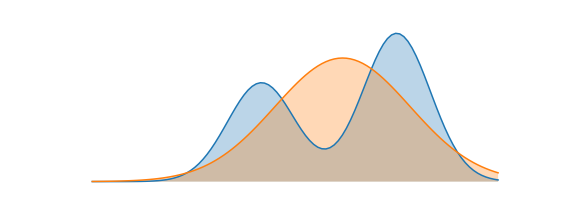
\includegraphics[scale=0.618]{pix/appendix/kl_forwardkl.png}
%\caption{Agent and Environment}
%\label{fig:label}
\end{figure}

\subsubsection{Reverse KL: Mode-Seeking Behaviour}

Now consider optimizing the reverse KL objective with respect to $q_\theta$
\begin{align*}
\arg\min_{\theta}D_{KL}(q \| p) &= \arg\min_{\theta} \mathbb{E}_{x \sim q_\theta}[-\log p(X)] - \mathcal{H}(q_\theta(X))\\
&= \arg\max_{\theta} \mathbb{E}_{x \sim q_\theta}[\log p(X)] + \mathcal{H}(q_{\theta}(X))
\end{align*}
Let's translate the objective above into words. The objective above will sample points 
from $q(X)$ and try to maximize the probability of these points under $p(X)$. The entropy 
term encourages the approximate distribution to be as wide as possible. A good approximation 
under the reverse KL objective thus satisfies
\begin{emp_box}
Wherever $q(\cdot)$ has high probability, $p(\cdot)$ must also have high probability.
\end{emp_box}\noindent
We consider this mode-seeking behaviour, because any sample from the approximate distribution 
$q$ must lie within a mode of $p$ (since it's required that samples from $q$ have high 
probability under $p$). Notice that unlike the forward KL objective, there's nothing 
requiring the approximate distribution to try to cover all the modes. The entropy term 
prevents the approximate distribution from collapsing to a very narrow mode; typically, 
behaviour when optimizing this objective is to find a mode of $p$ with high probability 
and wide support, and mimic it exactly.

The optimal "approximate" distribution for our example is shown below. Notice that the 
approximate distribution essentially encompasses the right mode of $p$. The reverse KL 
divergence does not penalize $q$ for not placing probability mass on the other mode of 
$p$.

\begin{figure}[H]
\centering
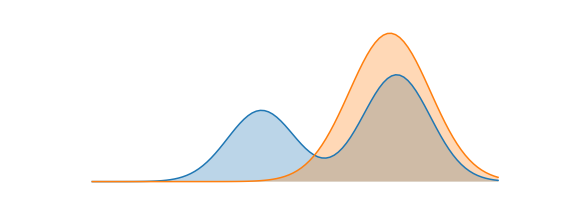
\includegraphics[scale=0.618]{pix/appendix/kl_reversekl.png}
%\caption{Agent and Environment}
%\label{fig:label}
\end{figure}


\subsubsection{Which one should I use?}

In this toy example, because we knew the exact distribution of $p$, we were able to show 
the behaviour of minimizing the forward and reverse KL divergences. In practice, it's 
often not possible to do both, and you are limited by domain to only one.

\noindent
{\bf FORWARD KL}

Recall that the simplified objective for the forward KL objective was
$$
\arg\max_{\theta} \mathbb{E}_{x \sim p}[\log q_\theta(X)]
$$
To be able to evaluate this objective, we need either a dataset of samples from the true 
model $p(X)$, or a mechanism for sampling from the true model.

\noindent
{\bf REVERSE KL}

The simplified objective for the forward KL objective was
$$
\arg\max_{\theta} \mathbb{E}_{x \sim q_\theta}[\log p(X)] + \mathcal{H}(q_{\theta}(X))
$$
To be able to evaluate this objective, we need to be able to evaluate probabilities of 
data-points under the true model $p(X)$.


%+++++++++++++++++++++++++++++++++++++++++++
\subsection{Supervised Learning = Forward KL}

Recall in supervised learning (empirical risk minimization), we have a dataset of samples 
$\mathcal{D} = \{(x_i,y_i)\}$ from some ground-truth data distribution $P(x,y) = P(x)P(y|x)$.

Our goal in supervised learning is to learn a model $f: \mathcal{X} \to \mathcal{Y}$ 
that minimizes the empirical risk of the model, which is parametrized by a loss function 
$L(f(x),y)$. In particular, we optimize over some distribution of models $f_\theta$
$$
\arg\min_{\theta} \mathbb{E}_{(x,y) \sim \mathcal{D}}[L(f_\theta(x),y)]
$$
We'll show that optimizing this objective is equivalent to minimizing the divergence from 
an approximate distribution $q_\theta(y|x)$ to the true data distribution $p(y|x)$. For 
reference, the forward KL divergence objective is
$$
\arg\min_{\theta} \mathbb{E}_{x,y \sim \mathcal{D}}[-\log Q_\theta(y|x)]
$$
%
\begin{itemize}
%\setlength{\itemsep}{0pt}
%\setlength{\parsep}{0pt}
\setlength{\parskip}{0pt}
\item[-]

{\bf Classification with Cross-Entropy Loss: }
Here, our approximate distribution $q_{\theta}(y|x)$ is a discrete distribution 
parametrized by a probability vector $p$ which is outputted by a neural network $f_\theta(x)$. 
By definition, the cross-entropy loss is exactly what the KL divergence minimizes.

\item[-]
{\bf Regression with Mean-Squared Error Loss: }
Here, our approximate distribution $q_{\theta}(y|x)$ is distributed normally 
$\mathcal{N}(f_{\theta}(x), I)$, where the mean of the distribution is parametrized by 
a neural network. The negative log-likelihood of the normal distribution is written below. 
Minimizing the NLL of this normal distribution is clearly equivalent to the mean-squared 
error loss.
$$
-\log q(y|x) = -\frac{1}{2}\|y - f_{\theta}(x)\|_2^2 + C
$$

\end{itemize}

This concept can in fact be extended to many other losses (for example, absolute error 
corresponds to the Laplace distribution). In particular, the forward KL divergence loss 
corresponds exactly to the problem of maximum-likelihood estimation which is the primary 
basis for many supervised learning problems.


%+++++++++++++++++++++++++++++++++++++++++++
\subsection{Reinforcement Learning = Reverse KL}
\label{Reinforcement-Learning-eq-Reverse-KL}

Viewing the problem of reinforcement learning as minimizing the reverse KL objective 
requires us to think about reinforcement learning from a probabilistic perspective. 
For a good intro on why we want to do that, and how exactly we formulate it, check out 
\nameref{Control-as-Inference}.

We can imagine that there's a distribution of optimal trajectories, given by 
$P_{opt}(\tau)$. Our goal in reinforcement learning is to learn stochastic policies 
$\pi(a|s)$ that induce a distribution over trajectories: $q_\pi(\tau)$. Now, we can't 
sample directly from the distribution of optimal trajectories $P_{opt}(\tau)$, but we 
know that the probability of a trajectory under optimality is exponential in the sum 
of rewards received on the trajectory.
$$
\log P(\tau) = \sum_{t=1}^T r(s_t,a_t)
$$
Optimizing the reverse KL objective then is
\begin{align*}
&~\arg\max_{\pi} \mathbb{E}_{\tau \sim Q_\pi}\left[\log P(\tau)\right] + \mathcal{H}(Q_{\pi}(\tau))\\
&=\arg\max_{\pi}\mathbb{E}_{\tau \sim Q_\pi}\left[\sum_{t=1}^T r(s_t,a_t)\right] 
+ \mathbb{E}_{\tau \sim Q_\pi}\left[\sum_{t=1}^T -\log \pi(a_t|s_t)\right]\\
&=\arg\max_{\pi}\mathbb{E}_{\tau \sim Q_\pi}\left[\sum_{t=1}^T \left(r(s_t,a_t) 
-\log\pi(a_t|s_t)\right)\right]\\
\end{align*}
This is exactly the maximum-entropy reinforcement learning objective!


%+++++++++++++++++++++++++++++++++++++++++++
\subsection{Summary}

KL divergences show up everywhere in machine learning, and a solid foundation in what 
the KL divergence measures is very useful. If you're interested in learning more about 
applications of KL divergence in statistics, I'd recommend reading articles on bayesian 
inference. KL divergence also has a very rich history in information theory: the 
following are great reads. If you love deep learning, two very important concepts in 
the field using KL divergences right now are VAEs and information bottlenecks.


%+++++++++++++++++++++++++++++++++++++++++++
\subsection{用途及实例}

{\bf 几个用途:}

\begin{itemize}
%\setlength{\itemsep}{0pt}
%\setlength{\parsep}{0pt}
\setlength{\parskip}{0pt}
\item[1.]
衡量两个概率分布的差异;

\item[2.]
衡量利用概率分布Q 拟合概率分布P 时的能量损耗,也就是说拟合以后丢失了多少的信息;

\item[3.]
衡量两个概率分布的相似度,在运动捕捉里面可以衡量未添加标签的运动与已添加标签运动的相似程度,
进而进行运动的分类。

\end{itemize}

DNN中最常使用的离散数值优化目标,莫过于交差熵。两个分布$p$,$q$的交差熵,
与KL距离实际上是同一回事。
$$
H(p,q) = -\sum p\log(q) = D_{KL}(p\parallel q) - \sum p\log(p)
$$
交差熵实际上就是KL距离减去熵,在深度学习框架中主要用来判定实际的输出与期望的输出的接近程度。

{\bf 例子:}
在做分类的训练的时候,如果一个样本属于第$K$类,那么这个类别所对应的的输出节点的输出值应该为$1$,
而其它节点的输出都为$0$,即$[0,0,1,0,\ldots, 0,0]$,这个数组也就是样本的Label,
是神经网络最期望的输出结果。也就是说用它来衡量网络的输出与标签的差异,
利用这种差异经过反向传播去更新网络参数。

\begin{example}
假设有一个字符发射器随机发射0和1两种字符,真实的发出概率分布为$A$,
但实际不知道$A$的具体分布。通过观察,得到概率分布$B$与$C$,各分布的具体情况如下:
\begin{align*}
A(0) &= 1/2, \quad A(1) = 1/2 \\
B(0) &= 1/4, \quad B(1) = 3/4 \\
C(0) &= 1/8, \quad C(1) = 7/8
\end{align}
通过计算得到:
\begin{align*}
KL(A\paralle B) &= 1/2 \log\frac{1/2}{1/4} + 1/2 \long\frac{1/2}{3/4} = 1/2\log(4/3)\\
KL(A\paralle C) &= 1/2 \log\frac{1/2}{1/8} + 1/2 \long\frac{1/2}{7/8} = 1/2\log(16/7)
\end{align}
由此可知,按照概率分布$B$进行编码,要比按照$C$进行编码,平均每个符号增加的比特数少。
从分布上也可以看出,实际上$B$要比$C$更接近真实分布(因为其与$A$分布的相对熵更小)。
\end{example}



%+++++++++++++++++++++++++++++++++++++++++++
\section{Maximum A Posteriori}
%-------------------------------------------
% https://zhuanlan.zhihu.com/p/184028576

最大后验估计则是贝叶斯推断的一个典型应用, 其强调将关于参数的先验知识带入到参数预估中, 
以达到对参数不确定性的建模, 在机器学习理论中充当参数正则化的角色。


%+++++++++++++++++++++++++++++++++++++++++++
\section{Maximum Likelihood Estimate}
%-------------------------------------------
% https://www.zhihu.com/question/484044429
% https://brilliant.org/wiki/maximum-likelihood-estimation-mle/

假设您建立了一个预测公司股价的模型。您注意到夜深人静的时候,股票价格上涨得很快。
背后可能有多种原因,找出可能性最大的原因便是最大似然估计的意义所在。
这一概念常被用于经济学、MRIs、卫星成像等领域。

最大似然估计以最大化观测数据集上的似然度为目标, 强调从观测数据集上拟合出产生观测数据集的分布, 
常用的交叉熵损失(cross entropy loss)、均方误差损失(Mean Square Error)都可以以最大似然估计作为其理论基础。


Maximum likelihood estimation (MLE) is a technique used for estimating the 
parameters of a given distribution, using some observed data. For example, 
if a population is known to follow a normal distribution but the mean and 
variance are unknown, MLE can be used to estimate them using a limited 
sample of the population, by finding particular values of the mean and 
variance so that the observation is the most likely result to have occurred.

MLE is useful in a variety of contexts, ranging from econometrics to MRIs 
to satellite imaging. It is also related to Bayesian statistics.

% https://brilliant.org/wiki/bayesian-theory-in-science-and-math/

在此节中,我们将研究最大似然估计(以下简称MLE)是如何工作的,
以及它如何用于确定具有任何分布的模型的系数。理解MLE将涉及到概率和数学,
但这里将尝试通过例子使它更通俗易懂。

{\bf 局限性:}\\
正态分布是缺省分布,也是最广泛使用的分布形式。
但如果采用其它更为正确的分布,则可以得到更好的结果。
最大似然估计是一种可以用于估计分布参数而不考虑所使用的分布的技术。
对于建模问题,首先要看看数据的分布情况,思考有没有比正态分布更有意义的分布。


%+++++++++++++++++++++++++++++++++++++++++++
\subsection{Basic concepts}

假设我们有观测数据集 $\mathcal{D}=\{x_i\}_{i=1}^n$, 如果我们希望通过预估参数 $\theta$ 来获得产生数据集 
$\mathcal{D}$ 的近似分布 $p_\text{model}(x;\theta)$, 一个非常自然的想法是既然数据集 $\mathcal{D}$ 
已经产生了, 何不让分布 $p_\text{model}(\mathcal{D};\theta)$ 最大化, 即使得分布 $p_\text{model}$ 
以最大概率产生观测数据集 $\mathcal{D}$ 中的数据, 这便是最大似然估计的指导思路。具体地, 我们有
\begin{align}
\mathcal{L}(\theta) &= \prod_{i=1}^n p_{\text{model}}(x_i; \theta) \\
\hat{\theta} &= \underset{\theta}{\operatorname{argmax}} \mathcal{L}(\theta) \notag
\end{align}
由于多个概率值进行连乘操作容易引起数值溢出的问题, 我们通常会求解等价问题
\begin{align}
\mathcal{N}(\theta) &= -\sum_{i=1}^n \log\left( p_{\text{model}}(x_i; \theta) \right) 
\label{eq_negative_log_likelihood} \\
\hat{\theta} &= \underset{\theta}{\operatorname{argmax}} \mathcal{N}(\theta) \notag
\end{align}
我们通常称 (\ref{eq_negative_log_likelihood}) 为负对数似然函数(Negative Log Likelihood), 
这在机器学习中是常用的损失函数。如果我们将产生观测数据集 $\mathcal{D}=\{x_i\}_{i=1}^n$ 的分布记为 
$\mathbf{X}\sim P_{\text{data}}$, 由大数定理可知, 当 $n\rightarrow\infty$ 时, 
独立同分布的随机变量所产生样本的算术平均值依概率收敛于期望, 故(2)可转化为




%+++++++++++++++++++++++++++++++++++++++++++
\subsection{为什么要使用最大似然估计(MLE)?}

假如想预测活动门票的销售情况,数据的直方图和密度如下:

\begin{figure}[H]
\centering
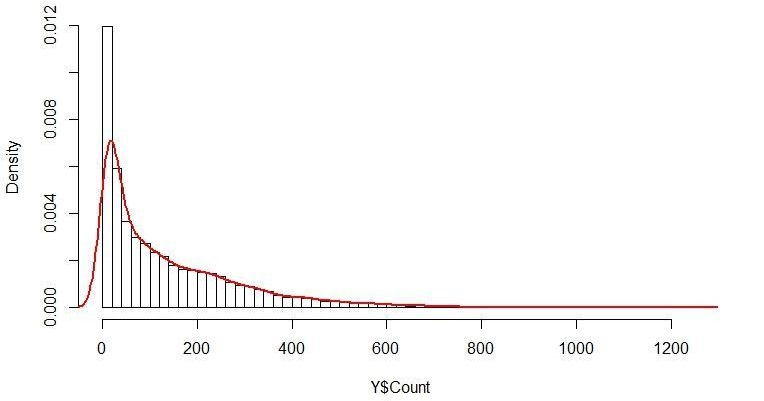
\includegraphics[scale=1.0]{pix/Histogram_of_Count_Variable.jpg}
\caption{Histogram of Count Variable}
%\label{fig:label}
\end{figure}

你将如何为这个变量建模?该变量不是正态分布的,而且是不对称的,因此不符合线性回归的假设。
一种常用的方法是对变量进行对数、平方根(sqrt)、倒数等转换,使转换后的变量服从正态分布,
并进行线性回归建模。让我们试试这些转换,看看结果如何。

{\bf 对数转换:}

\begin{figure}[H]
\centering
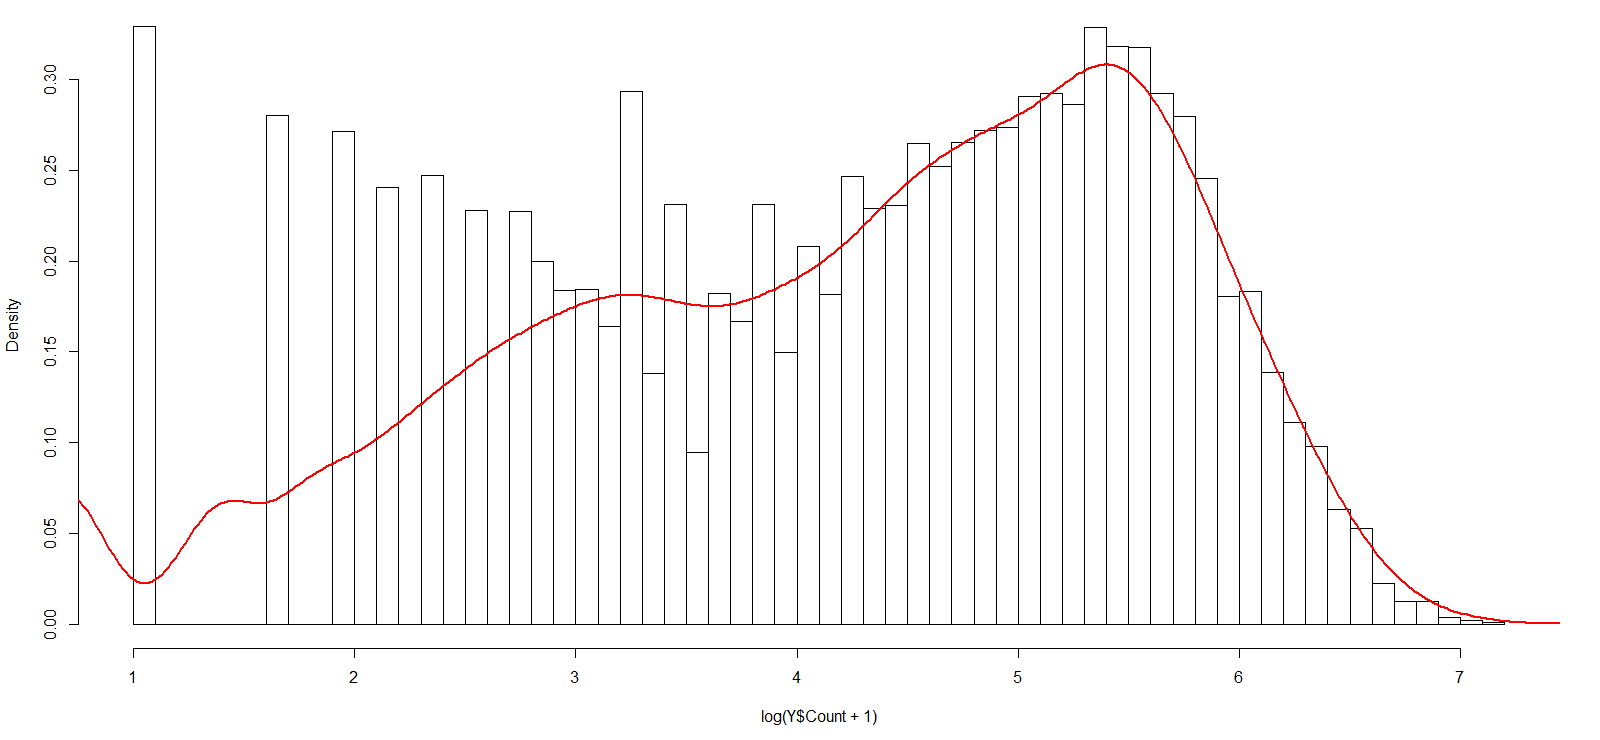
\includegraphics[scale=0.4]{pix/Histogram_of_Count_Variable_log.png}
\caption{Histogram of Count Variable: Log Trans}
%\label{fig:label}
\end{figure}

{\bf 平方根转换:}

\begin{figure}[H]
\centering
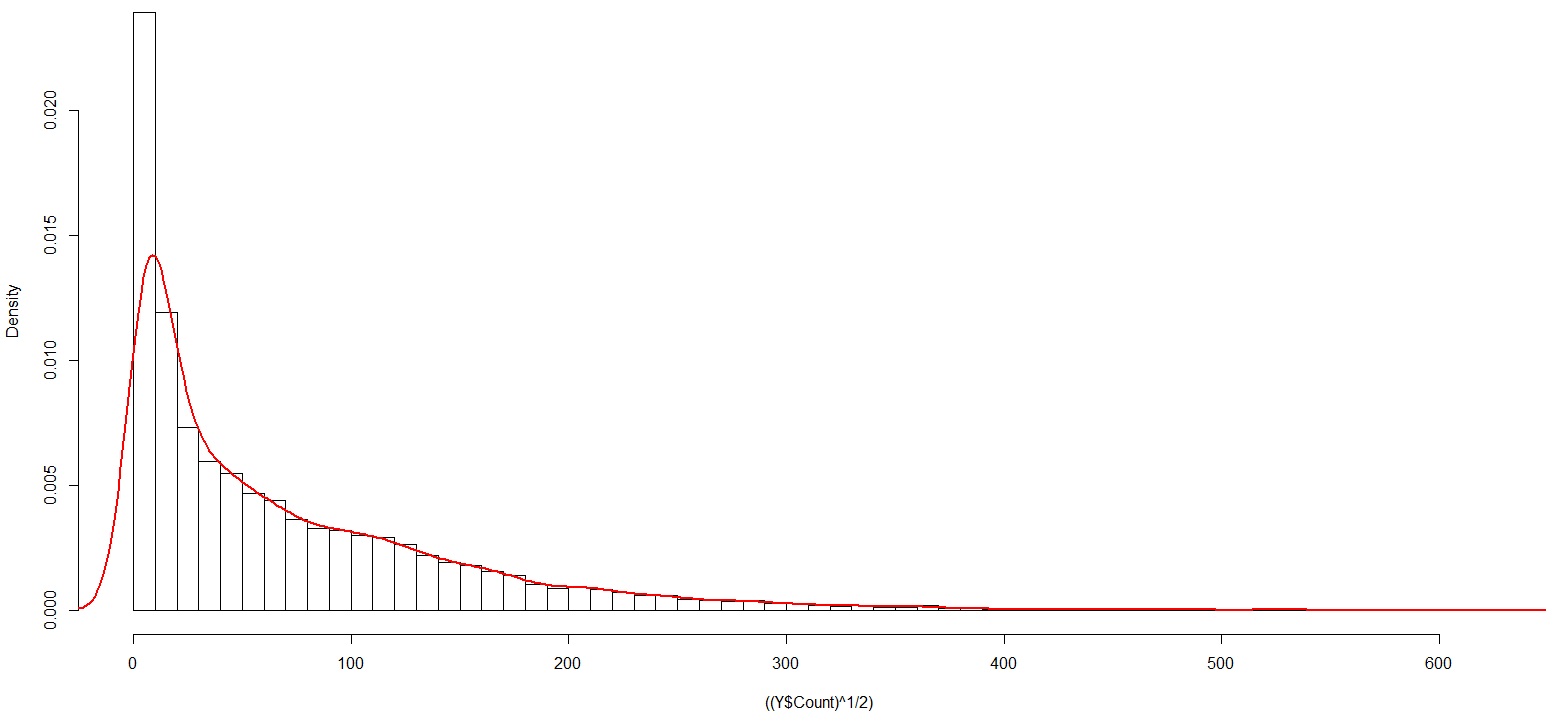
\includegraphics[scale=0.4]{pix/Histogram_of_Count_Variable_sr.png}
\caption{Histogram of Count Variable: Square Root}
%\label{fig:label}
\end{figure}

{\bf 倒数转换:}

\begin{figure}[H]
\centering
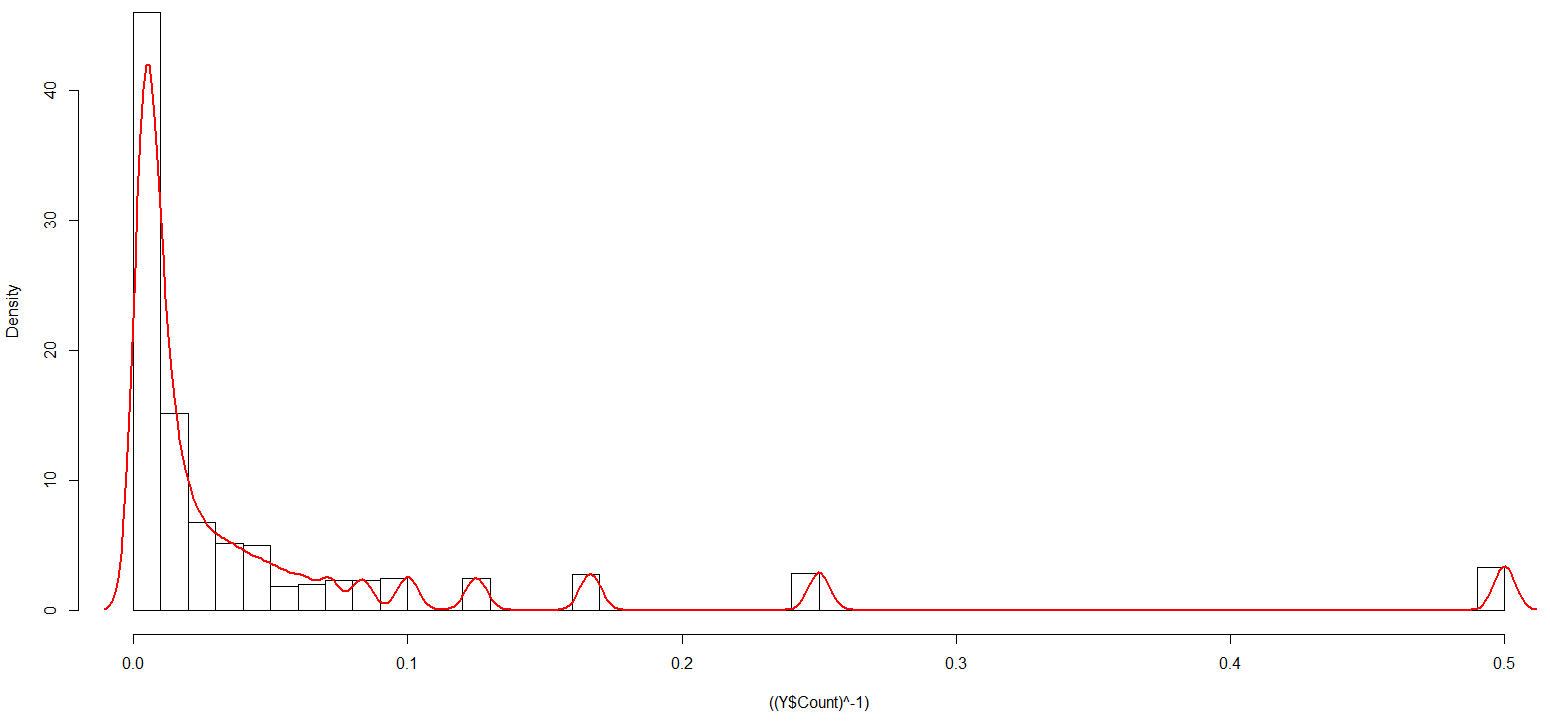
\includegraphics[scale=0.4]{pix/Histogram_of_Count_Variable_reciprocal.png}
\caption{Histogram of Count Variable: reciprocal}
%\label{fig:label}
\end{figure}

所有这些都不接近正态分布,那么我们应该如何对这些数据进行建模,才能不违背模型的基本假设?
如何利用正态分布以外的其他分布来建模这些数据呢?如果我们使用了不同的分布,又将如何来估计系数?
这便是最大似然估计(MLE)的主要优势。


\subsection{通过一个实例理解MLE}

在研究统计和概率时,你肯定遇到过诸如$x>100$的概率,因为$x$服从正态分布,平均值为$50$,
标准差为$10$。在这些问题中,我们已经知道分布(在这种情况下是正态分布)及其参数(均值和标准差),
但在实际生活问题中,这些参数是未知的,并且必须从数据中估计出来。
MLE可以帮助我们确定给定数据的分布参数。

下面用一个例子来加深理解:假设我们用数据来表示班级中学生的体重(以kg为单位)。
数据如下图所示(还提供了用于生成数据图的R代码):

\begin{figure}[H]
\centering
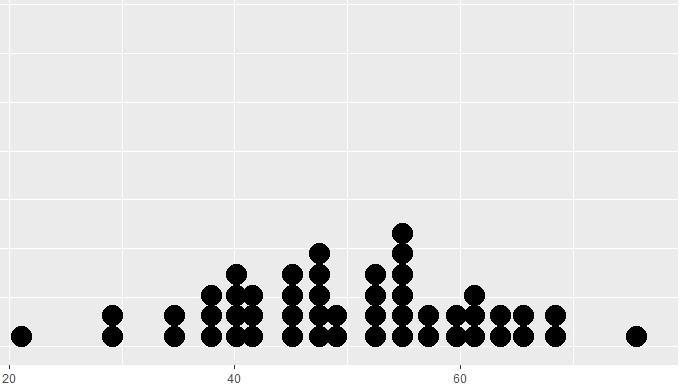
\includegraphics[scale=0.6]{pix/weights_of_students.jpg}
\caption{学生体重分布}
\label{fig:weights_of_students}
\end{figure}

\begin{lstlisting}[language=R]
x = as.data.frame(rnorm(50,50,10))
ggplot(x, aes(x = x)) + geom_dotplot()
\end{lstlisting}

这似乎遵循正态分布。但是我们如何得到这个分布的均值和标准差呢?
一种方法是直接计算给定数据的平均值和标准差,分别为49.8公斤和11.37公斤。
这些值能很好地表示给定的数据,但还不能最好地描述总体情况。

我们可以使用MLE来获得更稳健的参数估计。因此,
{\bf MLE可以定义为从样本数据中估计总体参数(如均值和方差、泊松率(Lambda)等)的方法,
从而使获得观测数据的概率(可能性)最大化。}

为了加深对MLE的理解,尝试猜测下列哪一项会使观察上述数据的概率最大化?

\begin{itemize}
%\setlength{\itemsep}{0pt}
%\setlength{\parsep}{0pt}
\setlength{\parskip}{0pt}

\item[(1)]
Mean = 100, SD = 10 均值=100,标准差=10

\item[(2)]
Mean = 50, SD = 10 均值=50 ,标准差=10

\end{itemize}

显然,如果均值为100,我们就不太可能观察到上述数据分布图形。



\subsection{进一步了解技术细节}

知道MLE能做什么之后,我们就可以深入了解什么是真正的似然估计,以及如何对它最大化。
首先,我们从快速回顾分布参数开始。

\subsubsection{分布参数}

首先,来了解一下分布参数。维基百科对这个词的定义如下:“它是一个概率分布的量化指数”,
可以将它视为样本总数的数值特征或一个统计模型。通过下面的图表来理解它:

\begin{figure}[H]
\centering
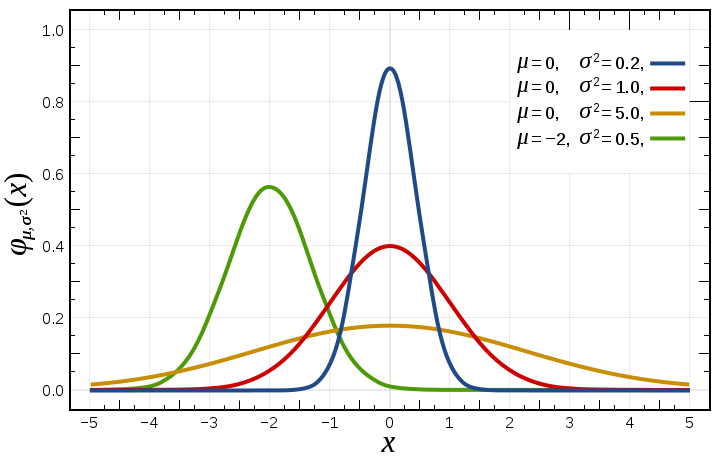
\includegraphics[scale=0.6]{pix/distributed_para.png}
\caption{分布参数}
\label{fig:distributed_para}
\end{figure}

钟形曲线的宽度和高度由两个参数决定-均值和方差。这就是正态分布的分布参数。同样,
泊松分布由一个参数lambda控制,即事件在时间或空间间隔内发生的次数

\begin{figure}[H]
\centering
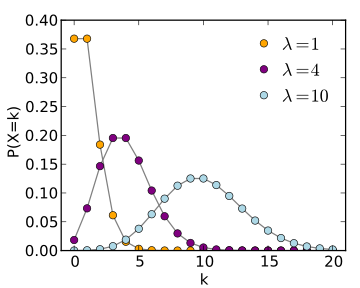
\includegraphics[scale=0.6]{pix/poison_distribution.png}
\caption{Poison Distribution}
\label{fig:poison_distribution}
\end{figure}

大多数分布都有一个或两个参数,但有些分布可以有多达4个参数,比如4参数β分布。


\subsubsection{似然}

我们先来直观理解一下极大似然(maximum-likelihood)背后的思想:
在只有概率的情况下,忽略低概率事件直接将高概率事件当作真实事件(的模型)的思想。

\begin{example}
{\bf 离散的小球问题:} \\
箱子里有一定数量的小球,每次随机拿取一个小球,查看颜色以后放回。
已知拿到白球的概率p为0.7或者0.3。假设现在已经拿了三次,都不是白球,
求拿到白球的概率的极大似然估计。
\end{example}

【{\bf 分析}】此处从数学上来讲,想要准确的求出拿到白球的概率是不可能的,
所以此处求的是概率的极大似然估计。而这里的有放回的拿取,是高中数学中经典的独立重复事件,
可以很简单的分别求出白球概率为0.7和0.3的时候拿三次都不是白球的概率。

【{\bf 解答}】\\
若拿到白球的概率为0.7,拿三次都不是白球的概率为:
$$
P_{0.7} = 0.3\times 0.3\times 0.3=0.027
$$

若拿到白球的概率为0.3,拿三次都不是白球的概率为:
$$
P_{0.3}=0.7\times 0.7\times 0.7=0.343
$$

由上:$P_{0.3}>P_{0.7}$,可知当前情况下白球概率为0.3的概率大于白球概率为0.7

综上所述:\\
拿到白球的概率的极大似然估计为0.3

% https://blog.csdn.net/a_rose_for_tang/article/details/106566430

极大似然估计的通常解法步骤:
\begin{itemize}
%\setlength{\itemsep}{0pt}
%\setlength{\parsep}{0pt}
\setlength{\parskip}{0pt}
\item[(1)]
得到所要求的极大似然估计的概率$p$的范围; 
\item[(2)]
以$p$为自变量,推导出当前已知事件的概率函数式$Q(p)$;
\item[(2)]
求出能使得$Q(p)$最大的$p$。
\end{itemize}
这样便求出了极大似然估计值$p$,就是已知数据求参数的方法。

最大似然估计是求参数$\theta$, 使似然函数$P(x_0|\theta)$最大($\theta$看为固定的)。
最大后验概率估计则是想求$\theta$使$P(x_0|\theta)P(\theta)$最大。
求得的$\theta$不单单让似然函数大,$\theta$自己出现的先验概率也得大。
($\theta$的概率不是固定的)

从图\ref{fig:distributed_para}和图\ref{fig:poison_distribution}中我们可以看到,
给定一组分布参数,一些数据值比其他数据的概率更大。从图\ref{fig:weights_of_students}中,
我们已经看到,当平均值是50而不是100时,给定的数据更有可能发生。然而,在现实中,
我们已经观察到了这些数据。因此,我们面临着一个逆向问题:给定观测数据和一个感兴趣的模型,
我们需要在所有概率密度中找到一个最有可能产生数据的概率密度函数/概率质量函数
$f(x_\theta)$。

为解决这一逆向问题,
我们通过逆转$f(x=\theta)$中的数据向量$x$和(分布)参数向量$\theta$来定义似然函数,即
$$
L(\theta; x) = f(x | \theta)
$$

在MLE中,可以假定我们有一个似然函数$L(\theta; x)$,其中$\theta$是分布参数向量,
$x$是观测集。我们感兴趣的是寻找具有给定观测值($x$值)的最大可能性的$\theta$值。


\subsubsection{对数似然}

如果假设观测集$\{x_i\}$是独立的同分布随机变量,
概率分布为$f_0$(其中$f_0$=正态分布,例如图\ref{fig:weights_of_students}),
那么手头的数学问题就变得简单了。似然函数可以简化为:
$$
L(\theta; x) = f_0(x_1, x_2, x_3, \ldots, x_n | \theta) = 
f_0(x_1 | \theta)\cdot f_0(x_2 | \theta)\cdot f_0(x_3 | \theta)\cdots
f_0(x_n | \theta)
$$

为了求这个函数的极大值/极小值,我们可以取此函数关于$\theta$的偏导数,
并将其设为$0$(极值位于驻点)。因为这里是乘积,所以需要用到求导的链式法则,
这对乘积来说是相当麻烦的。{\bf 一个聪明的诀窍是取似然函数的对数,并使其最大化。}
这将乘积转换为加法,并且由于对数是一个严格递增的函数,因此不会影响$\theta$的结果值。
所以我们有:
\begin{align*}
LL(\theta; x) &= \log\left[ 
f_0(x_1 | \theta)\cdot f_0(x_2 | \theta)\cdot f_0(x_3 | \theta)\cdots
f_0(x_n | \theta) \right] \\
&= \log f_0(x_1 | \theta) + \log f_0(x_2 | \theta) + \ldots 
+ \log f_0(x_n | \theta)
\end{align}


\subsubsection{最大似然估计}

为找到对数似然函数$LL(\theta; x)$的极大值,我们可以:

\begin{itemize}
%\setlength{\itemsep}{0pt}
%\setlength{\parsep}{0pt}
\setlength{\parskip}{0pt}
\item[-]
取$LL(\theta; x)$函数的一阶导数,并将其等于0

\item[-]
取$LL(\theta; x)$函数的二阶导数,并确认其为负值
\end{itemize}

在许多情况下,微积分对最大化似然估计没有直接帮助,但最大值仍然可以很容易地识别出来。
在寻找最大对数似然值的参数值时,没有任何东西比一阶导数等于零具有更为 “优先”或特殊的位置。
当需要估计一些参数时,它仅仅是一个方便的工具而已。

在通常情况下,能对函数求最大值的argmax的方法都可能适合于寻找log似然函数的最大值。
这是一个无约束的非线性优化问题.我们寻求一种优化算法以下列方式工作:
\begin{itemize}
%\setlength{\itemsep}{0pt}
%\setlength{\parsep}{0pt}
\setlength{\parskip}{0pt}
\item[1.]
从任意起始点可靠地收敛到局部最小化

\item[2.]
速度尽可能快
\end{itemize}

使用优化技术来最大化似然是非常常见的;
可以有多种方法来实现(比如:牛顿法、Fisher评分法、各种基于共轭梯度的方法、最陡下降法、
Nder-Mead型(单纯形)方法、BFGS法和多种其他技术)。

结果表明,当模型假设为高斯时,MLE估计等价于一般的最小二乘法。
你可以参考这里来证明它。



\subsection{利用MLE确定模型系数}

% https://www.zhihu.com/question/484044429


\subsection{R语言的MLE实现}

% https://www.zhihu.com/question/484044429




\section{Maximum Likelihood vs Maximum Entropy}

% https://zhuanlan.zhihu.com/p/137426616
% https://www.cnblogs.com/Hi-Simon/p/15101289.html


\subsection{relationship between Maximum Likelihood Estimation and the Maximum Entropy Principle}

% https://stats.stackexchange.com/questions/504117/is-there-a-relationship-between-maximum-likelihood-estimation-and-the-maximum-en

I know that both techniques can be used to estimate distribution from the 
data, but I didn't see anything in common between the two and I haven't 
found anything yet for the internet that relates the two.

Yes there is a connection. Namely, fitting maximum likelihood in exponential 
(Gibbs) family models is equivalent to doing maximum entropy with some 
constraints. Formally speaking, there is a primal-dual relationship between 
max entropy and max likelihood - see for example Section 3.6 in 
\href{https://www.nowpublishers.com/article/Details/MAL-001}{Wainwright and Jordan (2008)}.

To see why this is the case less formally (i.e. without going into convex 
analysis and dual representations) let's first look at the maximum entropy 
principle and its solution. The principle tells us to choose the distribution 
$p^*$ which is "consistent with the data" and has maximum entropy, i.e.

\begin{align}
p^* &= \arg\max_{p\in \mathcal{P}} H(p)  \notag \\
\text{subject to}\quad \mathbb{E}_p\phi_k(x) &= \hat{\mu}_k, \ \forall k=1, \ldots, K
\label{max_entropy_subject}
\end{align}
where $H(\cdot)$ is Shannon entropy, $\mathcal{P}$ is the set of all possible 
distributions and the constraints encode the aforementioned consistency with
data.

The optimal solution $p^*$ is of the form (e.g. see Section 3.1 in
\href{https://www.nowpublishers.com/article/Details/MAL-001}{Wainwright and Jordan (2008)}
or \href{https://en.wikipedia.org/wiki/Maximum_entropy_probability_distribution#Distributions_with_measured_constants}{Wikipedia}
or derive by introducing Lagrange multipliers)
%
\begin{equation}\label{form_optimal_solution}
p_\theta(x) \propto \exp\left\{
\sum_{k=1}^K \theta_k \phi_k (x)
\right\}
\end{equation}
%
where $\theta_k$ are chosen to satisfy the constraints.

Now suppose you do maximum likelihood, assuming a $k$-parameter exponential 
family for our data, i.e.
%
\begin{equation}\label{k-parameter-exponential}
p_\theta(x) = \exp\left\{
\sum_{k=1}^K \theta_k \phi_k (x) - A(\theta)
\right\}
\end{equation}
%
where the parameters $\{\theta_k\}$ are unknown, the functions $\{\phi_k\}$ 
are given (these are called sufficient statistics), and 
$A(\theta) = \log\left(\int \exp\left\{\sum_{k=1}^K \theta_k \phi_k(x)\right\}dx\right)$ 
is the log-normalising constant (aka log-partition function).

Note that Equation (\ref{k-parameter-exponential}) is of the same form as 
Equation (\ref{form_optimal_solution}). Hence, if we can show that the maximum 
likelihood solution satisfies the moment matching constraints 
(\ref{max_entropy_subject}) then we are done.

Start by writing the log-likelihood of $n$ datapoints, setting $\theta=\{\theta_k\}$ 
and $\phi(\cdot) = \{\phi_k(\cdot)\}$ for cleaner notation:
%
$$
\ell(\theta; x_{1:n}) = \sum_{i=1}^n \log p_\theta(x_i) = \sum_{i=1}^n \theta^T\phi(x_i) - nA(\theta),
$$
%
then differentiating and setting to zero gives us the maximum likelihood solution:
%
$$
\nabla_\theta A(\theta) = \frac{1}{n}\sum\phi(x_i).
$$
%
Finally note that the LHS $\nabla_\theta A(\theta) = \mathbb{E}_{p(\theta)}\phi(x)$, 
while the RHS is exactly its empirical average and so we recover the 
constraints (\ref{max_entropy_subject}).

{\bf 问:}

So in some sense maximum likelihood is a more general estimator, since it 
can fit arbitrary distributions, not just the exponential family.


{\bf 答:}

I think you can still apply max entropy to non-exponential family 
distributions (see eg 
\url{https://www.pnas.org/doi/10.1073/pnas.1320578110}), 
and I guess in these cases the two (ML and ME) might not give the same answer.



